\documentclass[11pt]{beamer}
\usetheme{Antibes}
\usepackage[utf8]{inputenc}
\usepackage[german]{babel}
\usepackage[T1]{fontenc}
\usepackage{amsmath}
\usepackage{amsfonts}
\usepackage{amssymb}
\usepackage{graphicx}
\author{Gruppe C14 \\ Julián Häck, Martin Koytek, Lars Wenning, \textbf{Erik Zimmermann}}
\usepackage{float}
\title{Mechanik}
\usepackage{multicol}
%\setbeamercovered{transparent} 
%\setbeamertemplate{navigation symbols}{} 
%\logo{} 
%\institute{} 
%\date{} 
%\subject{} 
\begin{document}

\begin{frame}
\titlepage
\end{frame}

\begin{frame}{Inhaltsverzeichnis}
\tableofcontents
\end{frame}

\section{Bestimmung der Erdbeschleunigung mit dem Pendel}
\subsection{Versuchsbeschreibung}
\begin{frame}{Versuchsbeschreibung}
\begin{figure}[H]
\centering
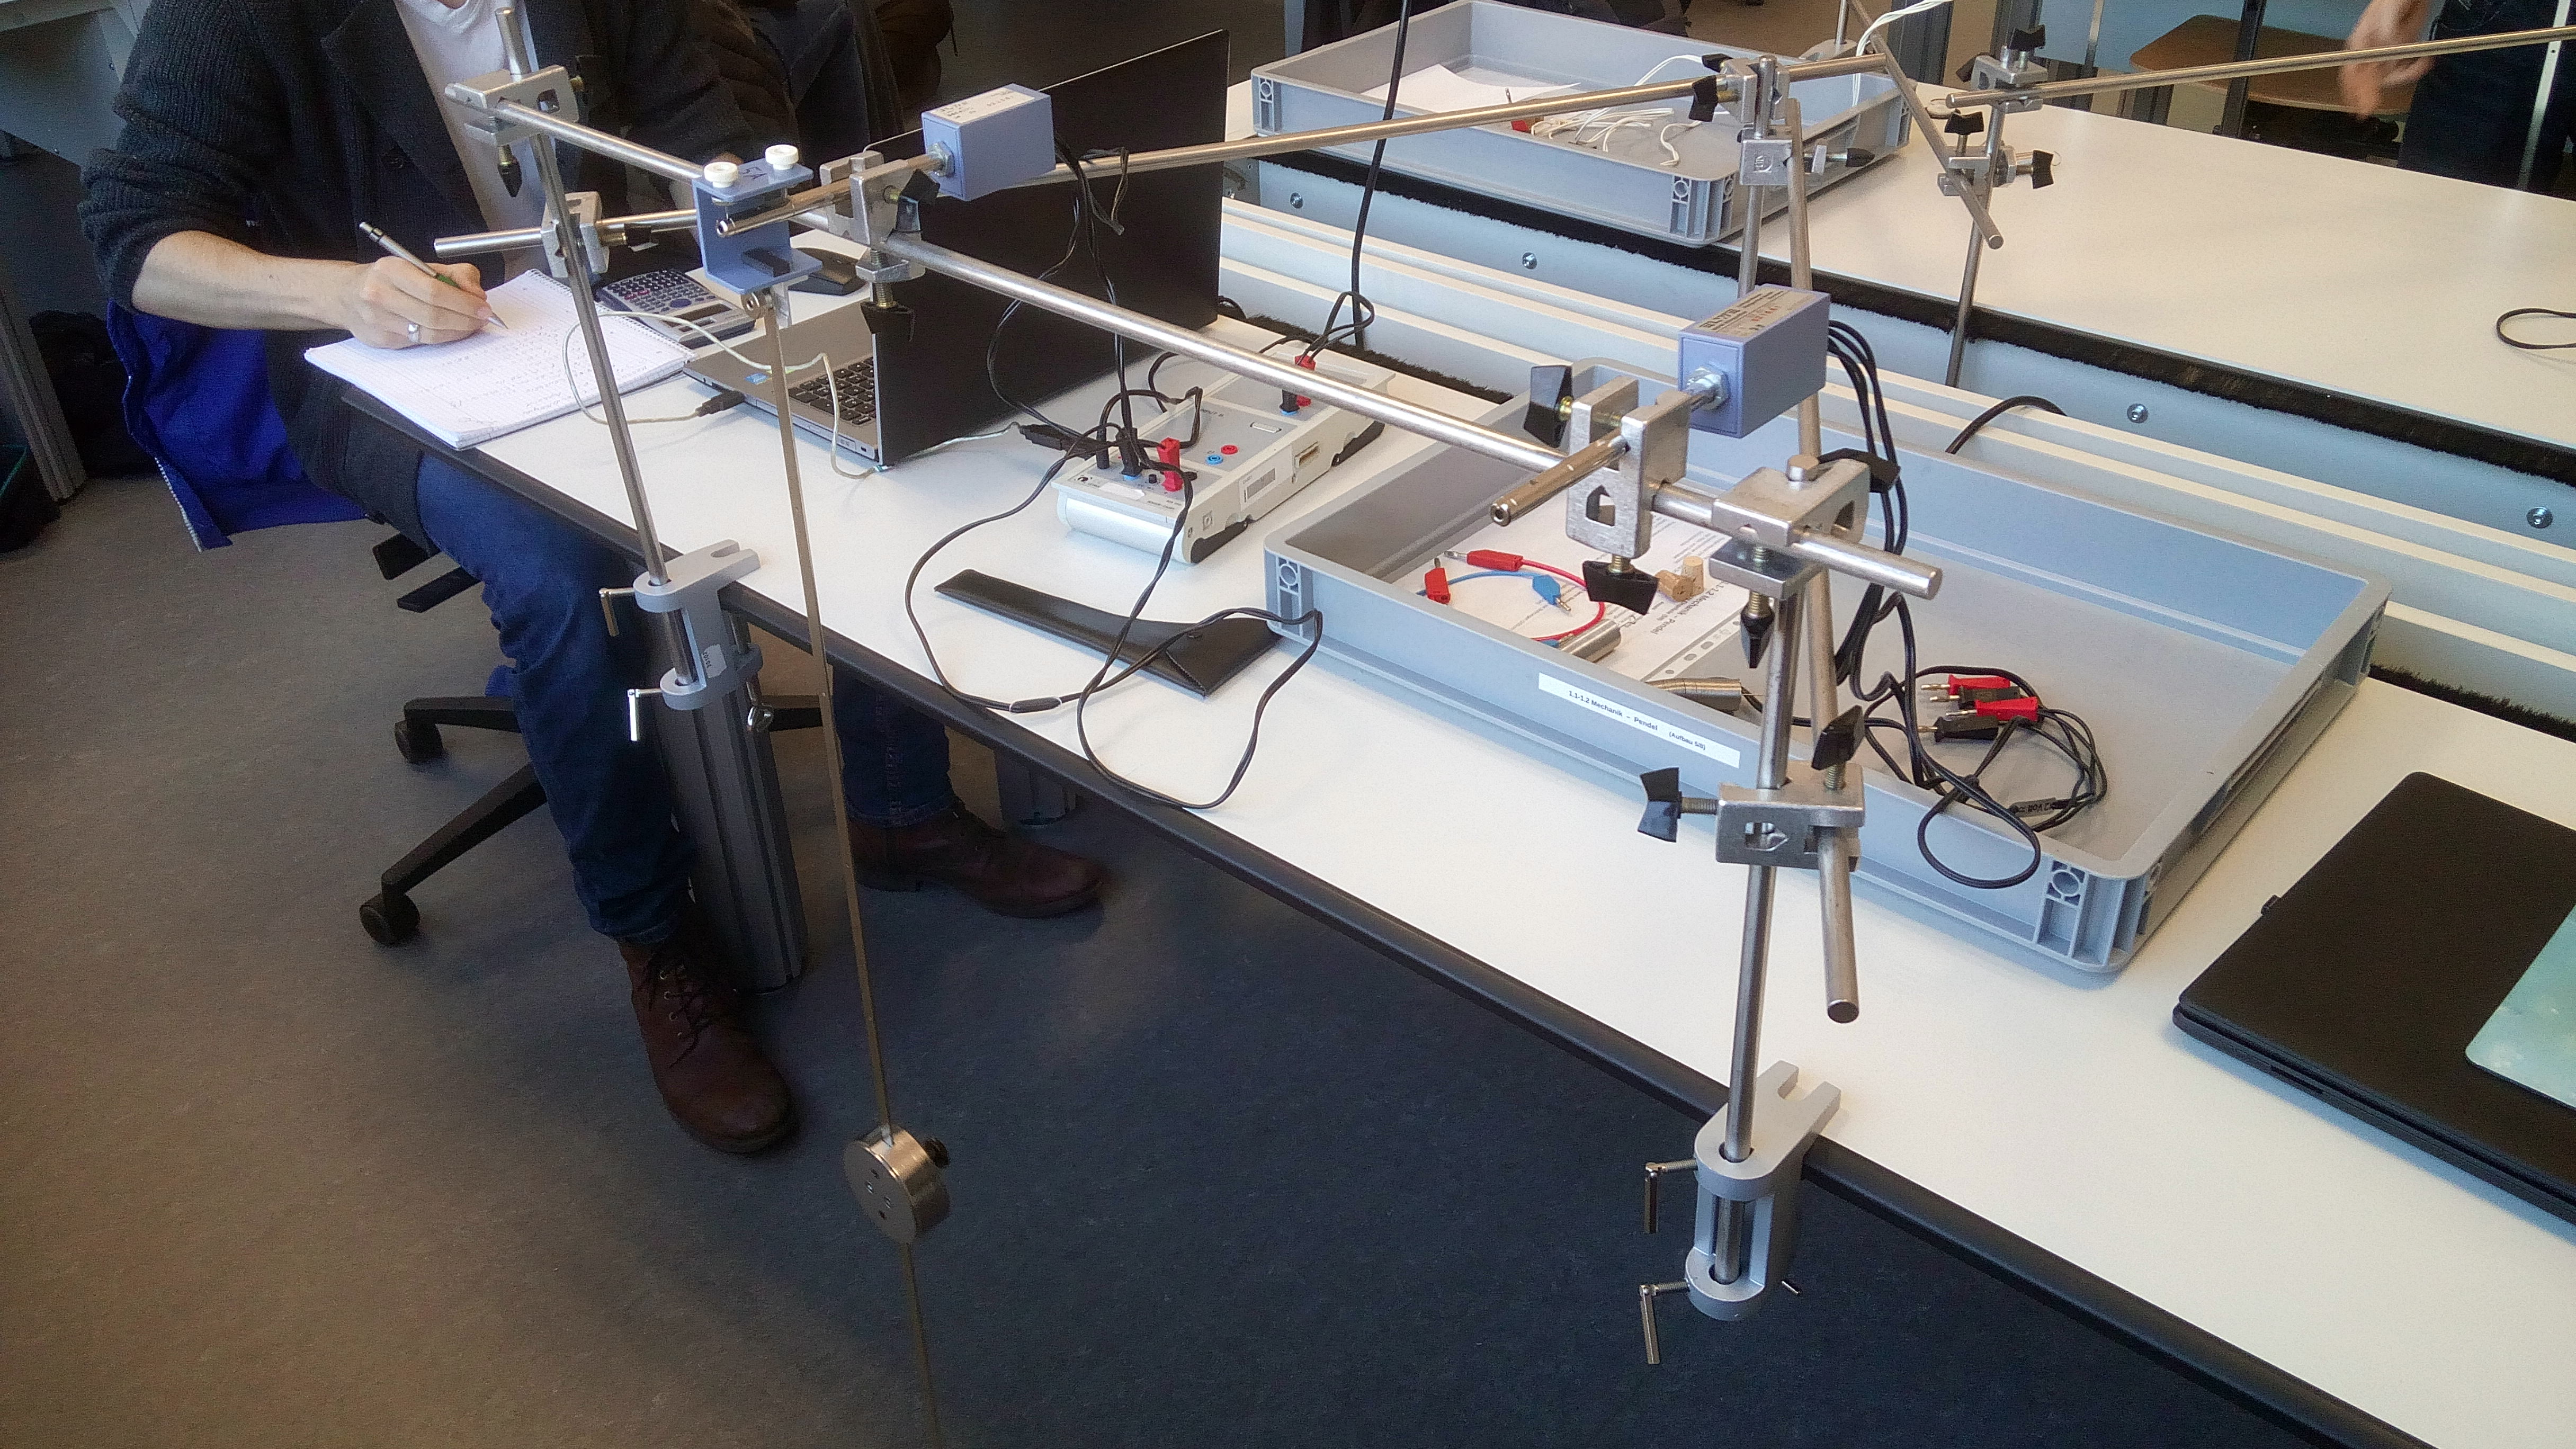
\includegraphics[scale=0.06]{Bilder/Einzelpendel.jpg}
\caption{Versuchsaufbau mit Pendelkörper}
\end{figure}
\end{frame}


\begin{frame}{Versuchsbeschreibung}
\begin{multicols}{2}
\begin{figure}[H]
\centering
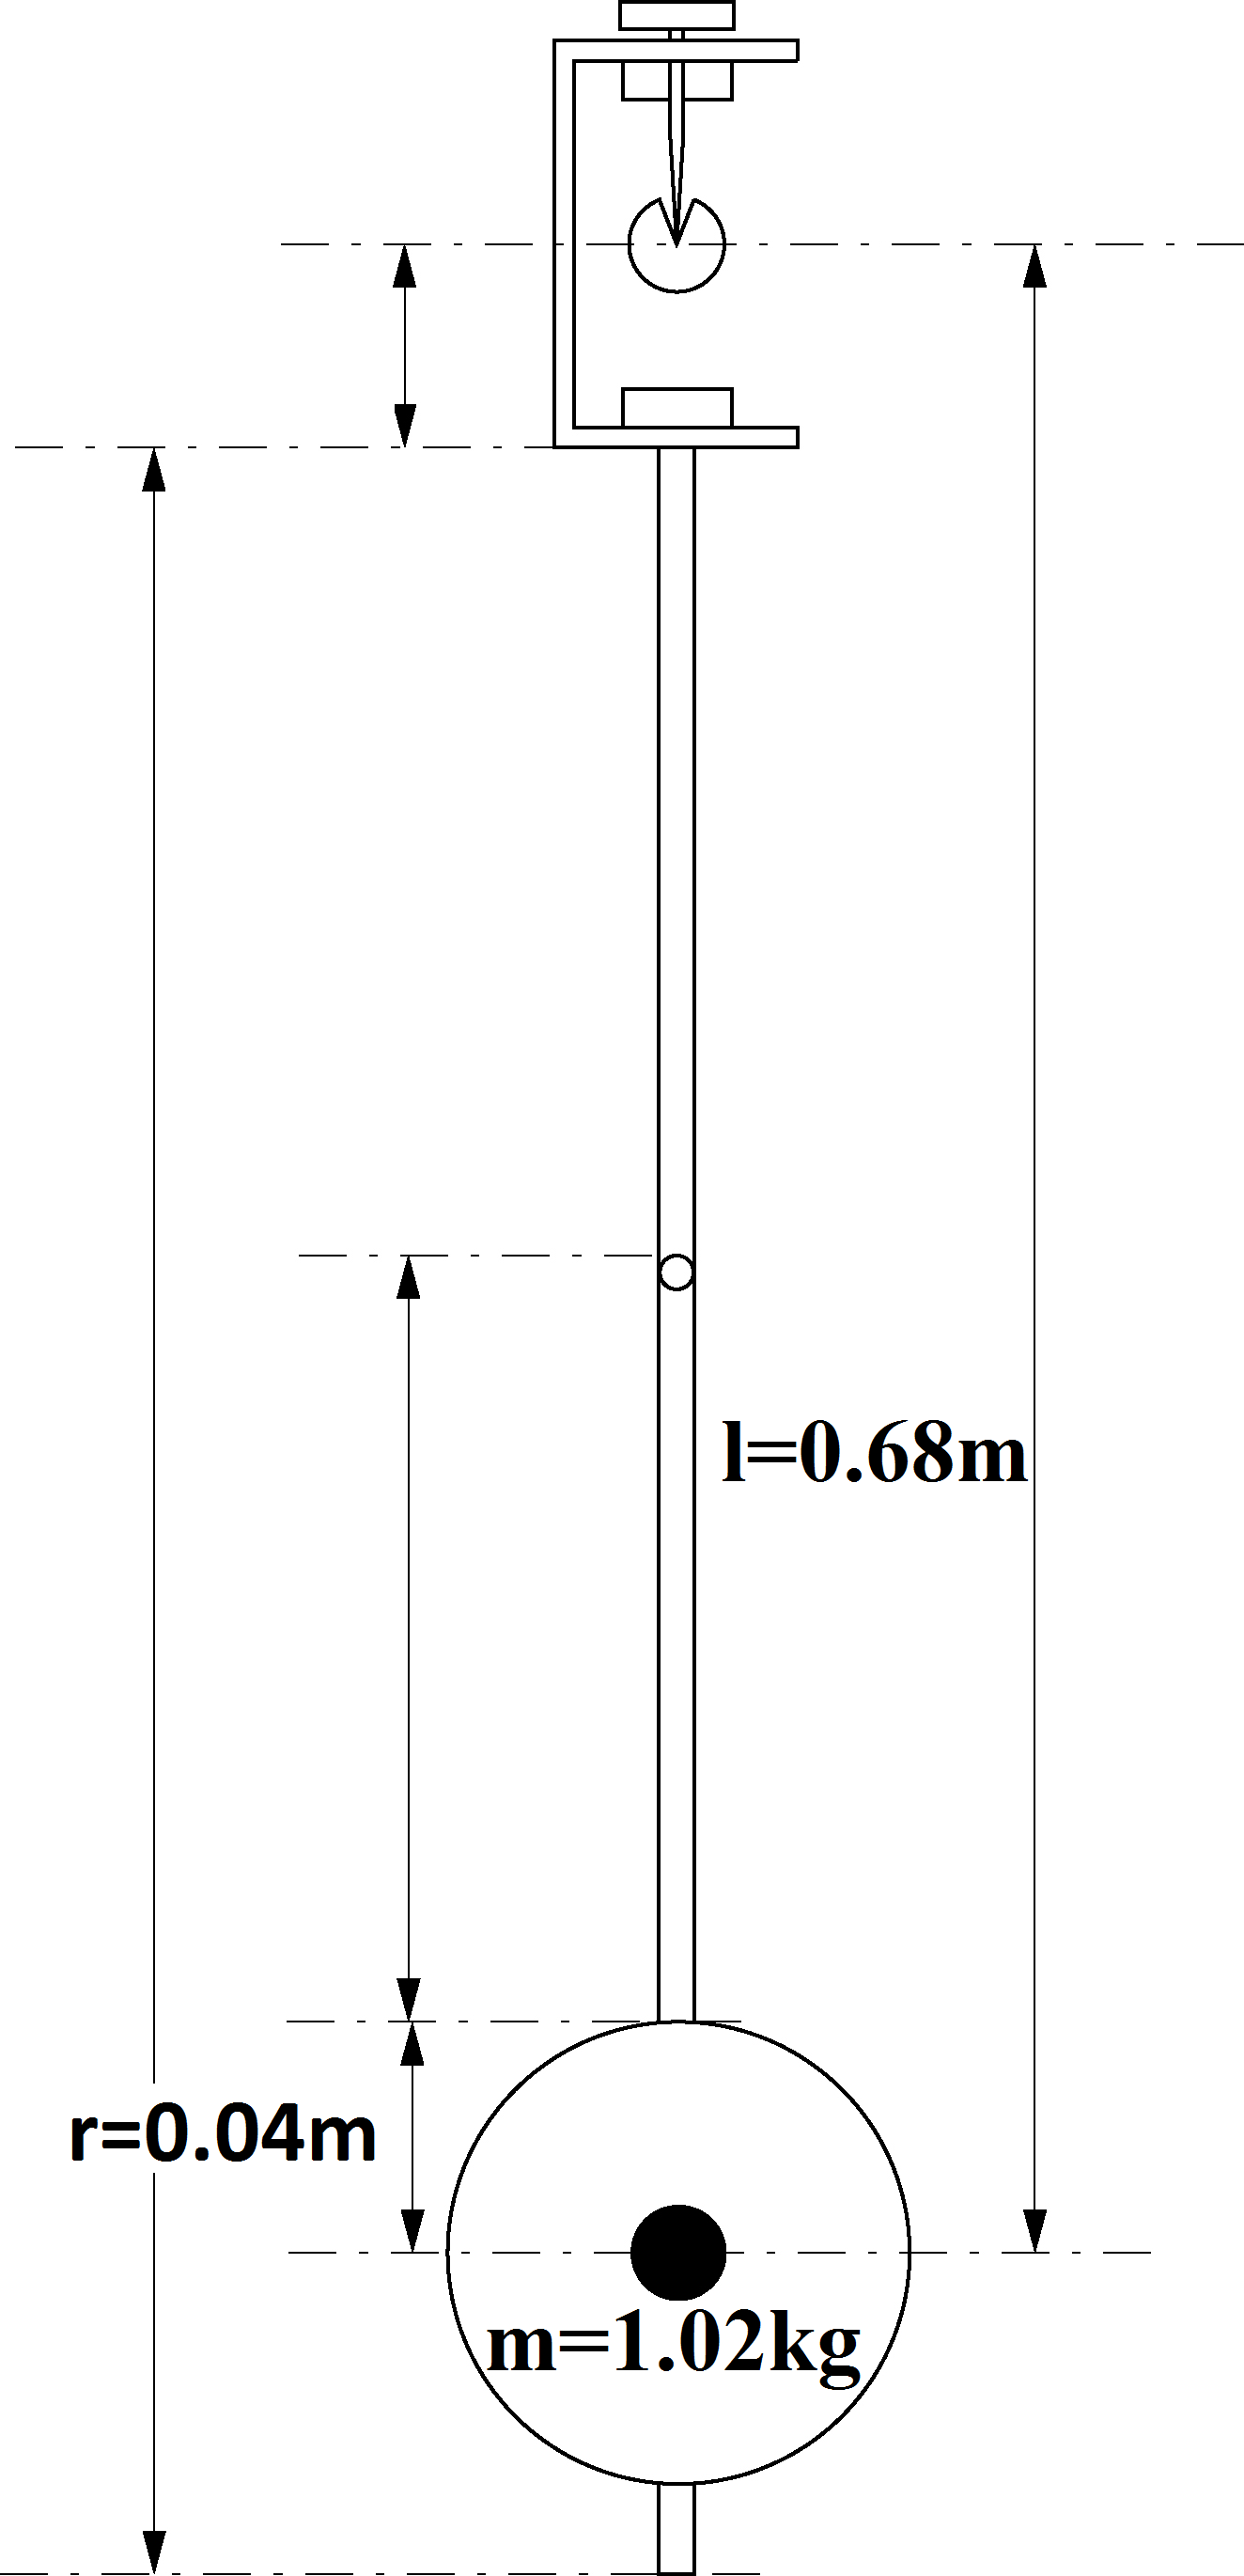
\includegraphics[scale=0.08]{Bilder/skizze_pendel_bearbeitet.png}
\end{figure}
\columnbreak
Mit
\begin{equation*}
\omega^2=\frac{D}{J}=\frac{m_p \cdot g \cdot l_p}{\frac{1}{2}m_p r_p^2+m_pl_p^2}
\end{equation*}
ergibt sich:
\begin{equation*}
g=\omega^2 l_p (1+\frac{r_p^2}{2 l_p^2}) 
\label{g}
\end{equation*} 
\end{multicols}
\end{frame}

\subsection{Rohdaten}
\begin{frame}{Rohdaten}
\begin{multicols}{2}
\begin{figure}[H]
\centering
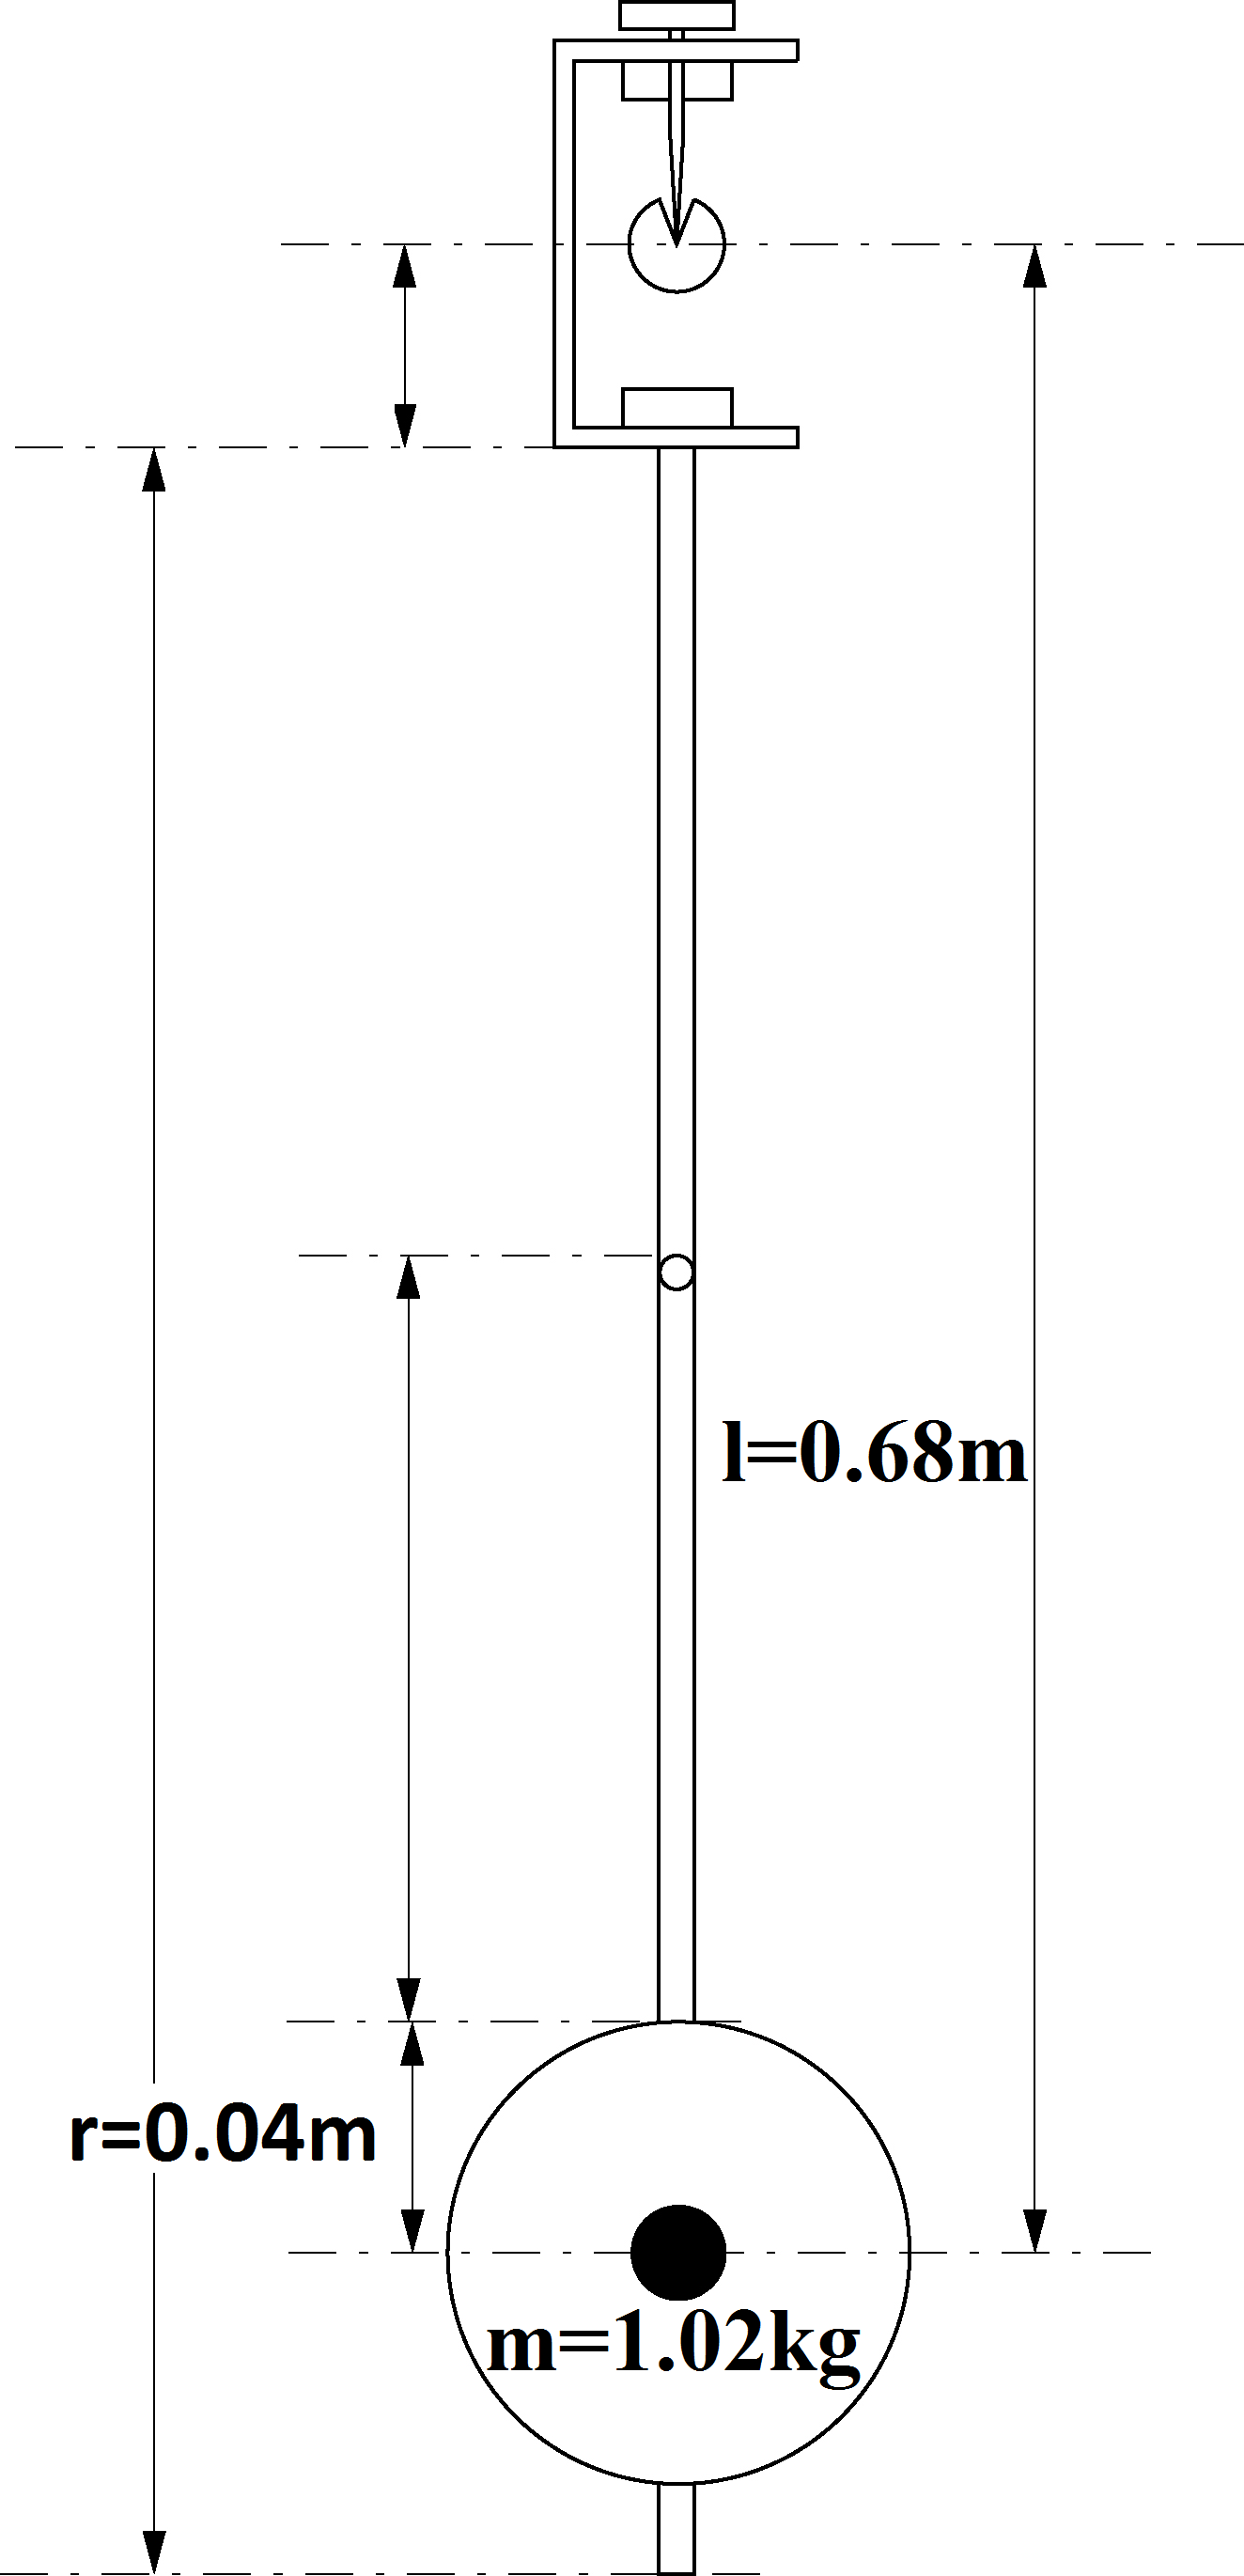
\includegraphics[scale=0.08]{Bilder/skizze_pendel_bearbeitet.png}
\end{figure}
\columnbreak
\begin{center}
\begin{tabular}{c|c|c}
 & Gruppe 1 & Gruppe 2 \\ 
\hline
Masse & 1.0207kg & 1.0217kg \\ 
$\sigma_{Masse}$ & 0.001kg & 0.001kg \\ 
D & 0.08m & 0.084m \\ 
$\Rightarrow$ Radius & 0.04m & 0.042m \\ 
$\sigma_{Schieblehre}$ & 0.0005m & 0.0005m \\ 
$l_p$ & 0.6788m & 0.689m \\ 
$\sigma_{l_p}$ & 0.01m & 0.01m \\ 
\hline
 & &  \\
$f_{ohne}$ [FFT] & 0.6039Hz & 0.6030Hz \\ 
$f_{mit}$ [FFT] & 0.6032Hz & 0.6011Hz \\ 
\end{tabular} 
\end{center}
\end{multicols}
\end{frame}

\subsection{Transformation der Rohdaten}
\begin{frame}{Transformation der Rohdaten}
\begin{figure}[H]
\centering
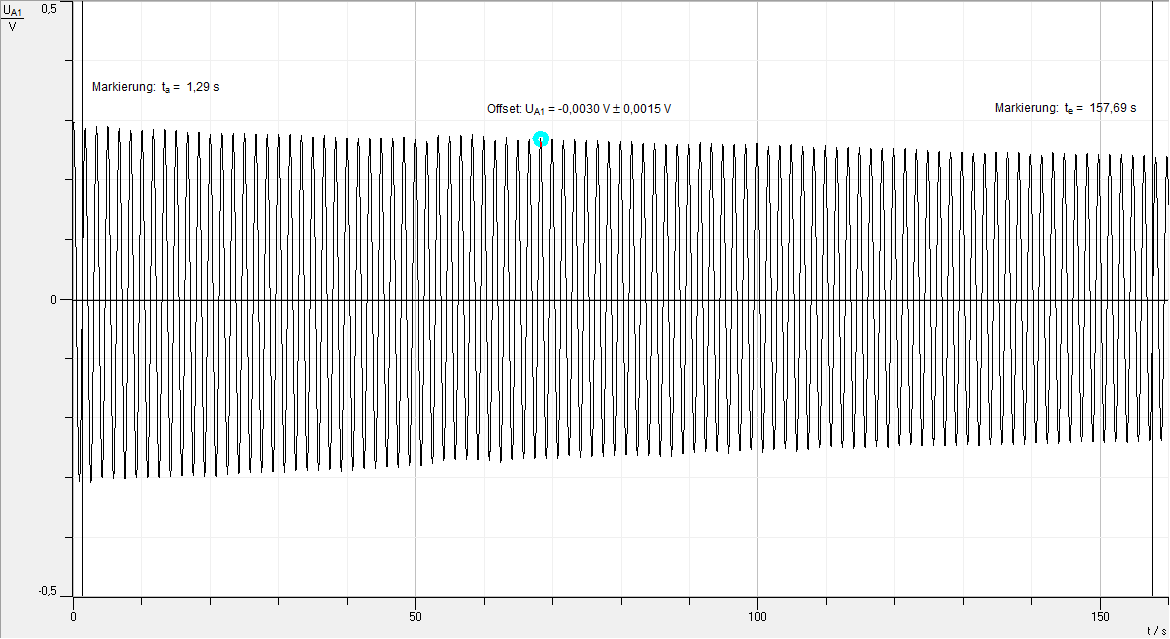
\includegraphics[scale=0.3]{Bilder/Erdbeschleunigung_bestimmungF.png}
\end{figure}
Hier:
\begin{equation*}
t_a=1.29s, \hspace{1cm} t_e=157.69s, \hspace{1cm} n=94, \hspace{1cm} \sigma_t=\frac{0.01}{\sqrt{12}}s
\end{equation*}
\end{frame}

\begin{frame}{Transformation der Rohdaten}
\begin{equation*}
\omega=\frac{2\pi n}{t_e-t_a}
\end{equation*}
\begin{equation*}
\sigma_{\omega}=\frac{2\cdot \pi \sqrt{2}\cdot n \cdot \sigma_t}{(t_e-t_a)^2}
\end{equation*}
\begin{equation*}
g=\omega^2 l_p (1+\frac{r_p^2}{2 l_p^2}) 
\end{equation*}
\begin{equation*}
\sigma_g=\sqrt{(2\omega l_p (1+\frac{r_p^2}{2 l_p^2}))^2 \cdot \sigma_{\omega}^2+(\omega^2 \cdot \frac{r_p}{l_p})^2 \cdot \sigma_r^2+(\omega^2(1-\frac{r_p^2}{2 l_p^2}))^2 \cdot \sigma_l^2} 
\end{equation*}
\end{frame}

\subsection{Ergebnisse}
\begin{frame}{Ergebnisse}
\begin{figure}[H]\centering
\begin{tabular}{c|c|c|c|c}
Messung: & 1. & 2. & 3. & 4. \\ 
g: Gruppe 1 & 9.766 & 9.766 & 9.770 & / \\ 
$\sigma_g$: Gruppe 1 & 0.071 & 0.072 & 0.072 & / \\ 
g: Gruppe 2 & 9.838 & 9.839 & 9.842 & 9.845 \\ 
$\sigma_g$: Gruppe 2 & 0.142 & 0.142 & 0.142 & 0.142 \\ 
\end{tabular} 
\newline
\newline
\end{figure}
gewichtet Gemittelt:
\begin{center}
\begin{tabular}{c|c|c}
 & Gruppe 1 & Gruppe 2 \\ 
\hline 
$\bar{g}$ & 9.767 & 9.841 \\ 
$\sigma_{\bar{g}}$ & 0.041 & 0.071 \\ 
\end{tabular} 
\newline
\newline
Angaben in $\frac{m}{s^2}$
\end{center}
\end{frame}

\subsection{Fazit}
\begin{frame}{Fazit}
\begin{center}
\begin{figure}[H]
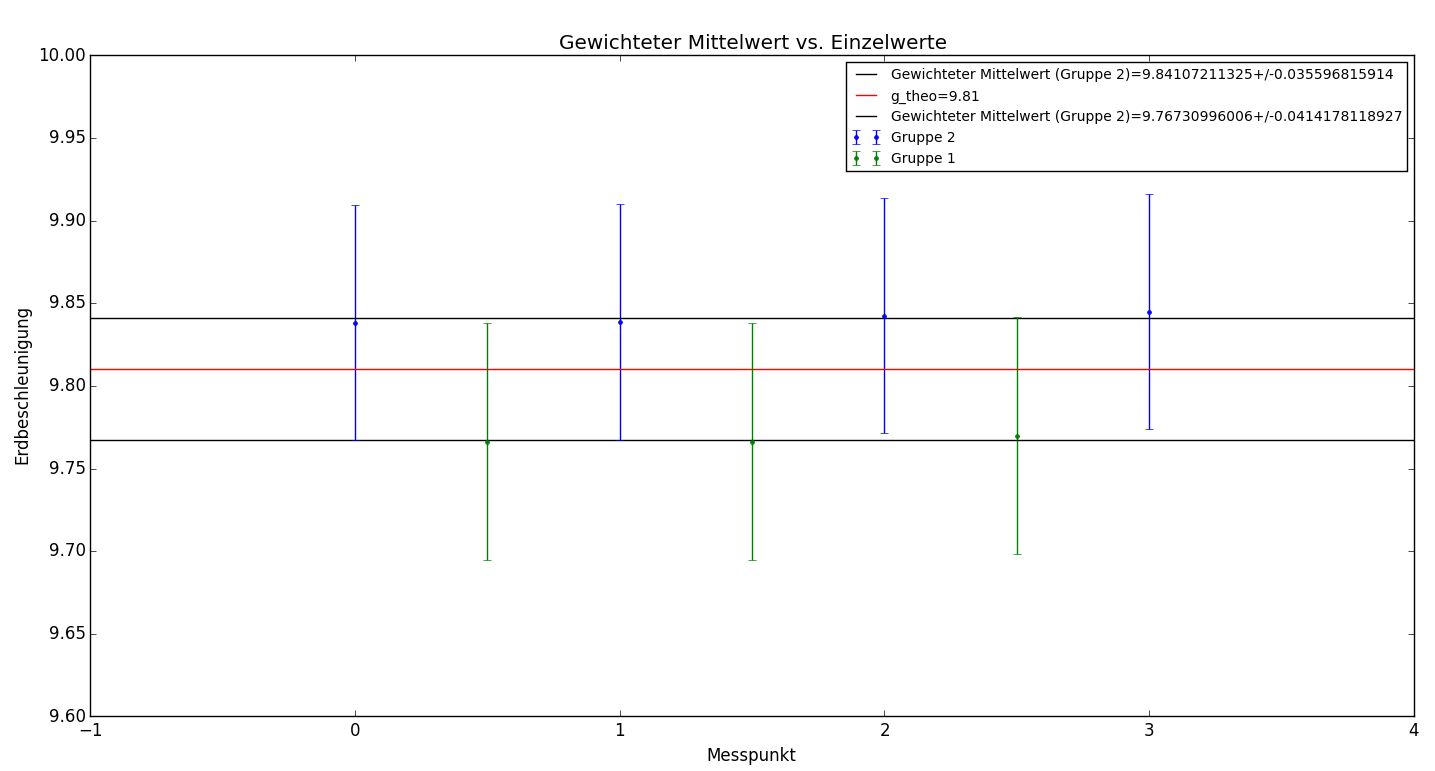
\includegraphics[scale=0.3]{Bilder/Erdbeschleunigung_alle_bearb.png}
\end{figure}
\end{center}
\end{frame}


\end{document}